\documentclass[10pt,a4paper]{article}
\setlength{\headheight}{14.49998pt}
\addtolength{\topmargin}{-2.49998pt}
% \usepackage{fontspec}
% \setsansfont{CMU Sans Serif}%{Arial}
% \setmainfont{CMU Serif}%{Times New Roman}
% \setmonofont{CMU Typewriter Text}%{Consolas}
\usepackage{scalerel,graphicx,xparse}
\usepackage{float}
\usepackage{microtype}
\usepackage{tikz}
\usetikzlibrary{decorations}
\usepackage{pygmentex}
\usepackage{pygmentize}
\usepackage{graphicx}
\usepackage{tikz}
\usepackage{enumitem}
\usepackage{subcaption}
\usepackage[version=4]{mhchem}
\usepackage{amsfonts} 
\usepackage{amssymb}
\usepackage{hyphenat}
\usepackage[breaklinks]{hyperref}
\usepackage[l3]{csvsimple}
\usepackage{amsmath}
\usepackage{lastpage}
\usepackage{fancyhdr}
\usepackage{multicol}
\usepackage{svg}
\usepackage{chemfig}
\usepackage{titlesec}
\usepackage{minted}
\usepackage{caption}
% \usepackage{subcaption}
\usepackage[table,dvipsnames]{xcolor} %deleted something from here (xcdraw)
\usepackage{cancel}
\usepackage{soul}
\usepackage{mol2chemfig}
\usepackage{amsmath,amssymb}
\usepackage{pdfpages}
\usepackage{tcolorbox}
\usepackage[title]{appendix}
\usepackage[a4paper,margin=2cm]{geometry}
\tcbuselibrary{minted,breakable,xparse,skins}

\DeclareTCBListing{mintedbox}{O{}m!O{}}{%
  breakable=true,
  listing engine=minted,
  listing only,
  minted language=#2,
  minted style=default,
  minted options={%
    linenos,
    gobble=0,
    breaklines=true,
    breakafter=,,
    fontsize=\small,
    numbersep=8pt,
    #1},
  boxsep=0pt,
  left skip=0pt,
  right skip=0pt,
  left=35pt,
  right=0pt,
  top=3pt,
  bottom=3pt,
  arc=5pt,
  leftrule=0pt,
  rightrule=0pt,
  bottomrule=2pt,
  toprule=2pt,
  colback=Lavender!15,
  colframe=Lavender,
  enhanced,
  overlay={%
    \begin{tcbclipinterior}
    \fill[Lavender!50!white] (frame.south west) rectangle ([xshift=30pt]frame.north west);
    \end{tcbclipinterior}},
  #3}

\AtBeginEnvironment{quote}{\itshape}
\definecolor{brilliantrose}{rgb}{1.0, 0.33, 0.64}
\hypersetup{
    colorlinks=true,
    linkcolor=brilliantrose,
    filecolor=magenta,      
    urlcolor=cyan,
    pdftitle={Overleaf Example},
    pdfpagemode=FullScreen,
    }

\urlstyle{same}
\newcommand{\titlestr}{Assignment 1}
\newcommand{\shorttitlestr}{MECH ENG 4106 Assignment 1}
\newcommand{\authorstr}{Mei He} % INSERT YOUR NAME(S)
\usepackage[backend=biber,style=chem-acs]{biblatex}
\addbibresource{bib_file.bib}
\usepackage[version=4]{mhchem}
\newcommand{\appendixpagenumbering}{
  \break
  \pagenumbering{roman}
  \renewcommand{\thepage}{\arabic{page}}
  \rfoot{Page \thepage\ of \pageref{LastPage}}
}
% Set better bond appearance
\setchemfig{
    atom sep=2.2em,
    bond style={line width=1pt},
    cram width=3pt,
    cram dash width=0.4pt
}
\titleformat*{\section}{\normalsize\bfseries}
\titleformat*{\subsection}{\normalsize\bfseries}
\titleformat*{\subsubsection}{\large\bfseries}
\titleformat*{\paragraph}{\large\bfseries}
\titleformat*{\subparagraph}{\large\bfseries}
\begin{document}
\sethlcolor{Lavender}
\newcommand{\mathcolorbox}[2]{\colorbox{#1}{$\displaystyle #2$}}
\renewcommand{\thesubsection}{(\alph{subsection})}
\renewcommand{\thesection}{\arabic{section}.}

%%%%%%%%%%%%%%%%%%%%%%%%%%%%%%555
% title page
\begin{titlepage}
  \centering
  \vspace*{\fill}
  
  {\LARGE \bf \titlestr \par}

  \vspace{0.3cm}
  {\large \authorstr \par}

  {\bf A1900510}

  \vspace{0.3cm}
  Submitted April 8th 2025     % PUT YOUR DATE HERE

  \vspace{0.5cm}
  Assignment submitted for
  {\bf Aerospace Propulsion}
  at the University of Adelaide.
  \\\textbf{Due 23:59pm April 11th 2025} %CHECK WHEN DUE
  
  \vspace{0.5cm}
  
\noindent\rule[6pt]{\linewidth}{0.4pt}
  \textbf{\large{Please see \hyperlink{email}{email evidence of extension}, and \hyperlink{accessplan}{access plan} at the end of this document}}
    % \begin{abstract}
    % % \input{0_abstract}
    % \end{abstract}
  \vspace{\fill}

\end{titlepage}
\begin{titlepage}
    \tableofcontents
    \listoffigures
\end{titlepage}

% put headings on each page
\pagestyle{fancy}
\fancyhf{}
\rhead{\shorttitlestr}
\lhead{\authorstr}
\rfoot{Page \thepage\ of \pageref{lastcontentpage}}
\renewcommand{\headrulewidth}{1pt}

%%%%%%%%%%%%%%%%%%%%%%%%%%%%%%555
% main report
\clearpage

%%%%%%%%%%%%%%%%%%%%%%%%%%%%%%555
% q1

\input{q1/q1}
%%%%%%%%%%%%%%%%%%%%%%%%%%%%%%555
% q1
\input{q2/q2}
%%%%%%%%%%%%%%%%%%%%%%%%%%%%%%555
% q1
\input{q3/q3}
%%%%%%%%%%%%%%%%%%%%%%%%%%%%%%555
% q1

\input{q4/q4}
\label{lastcontentpage}
\hypertarget{email}{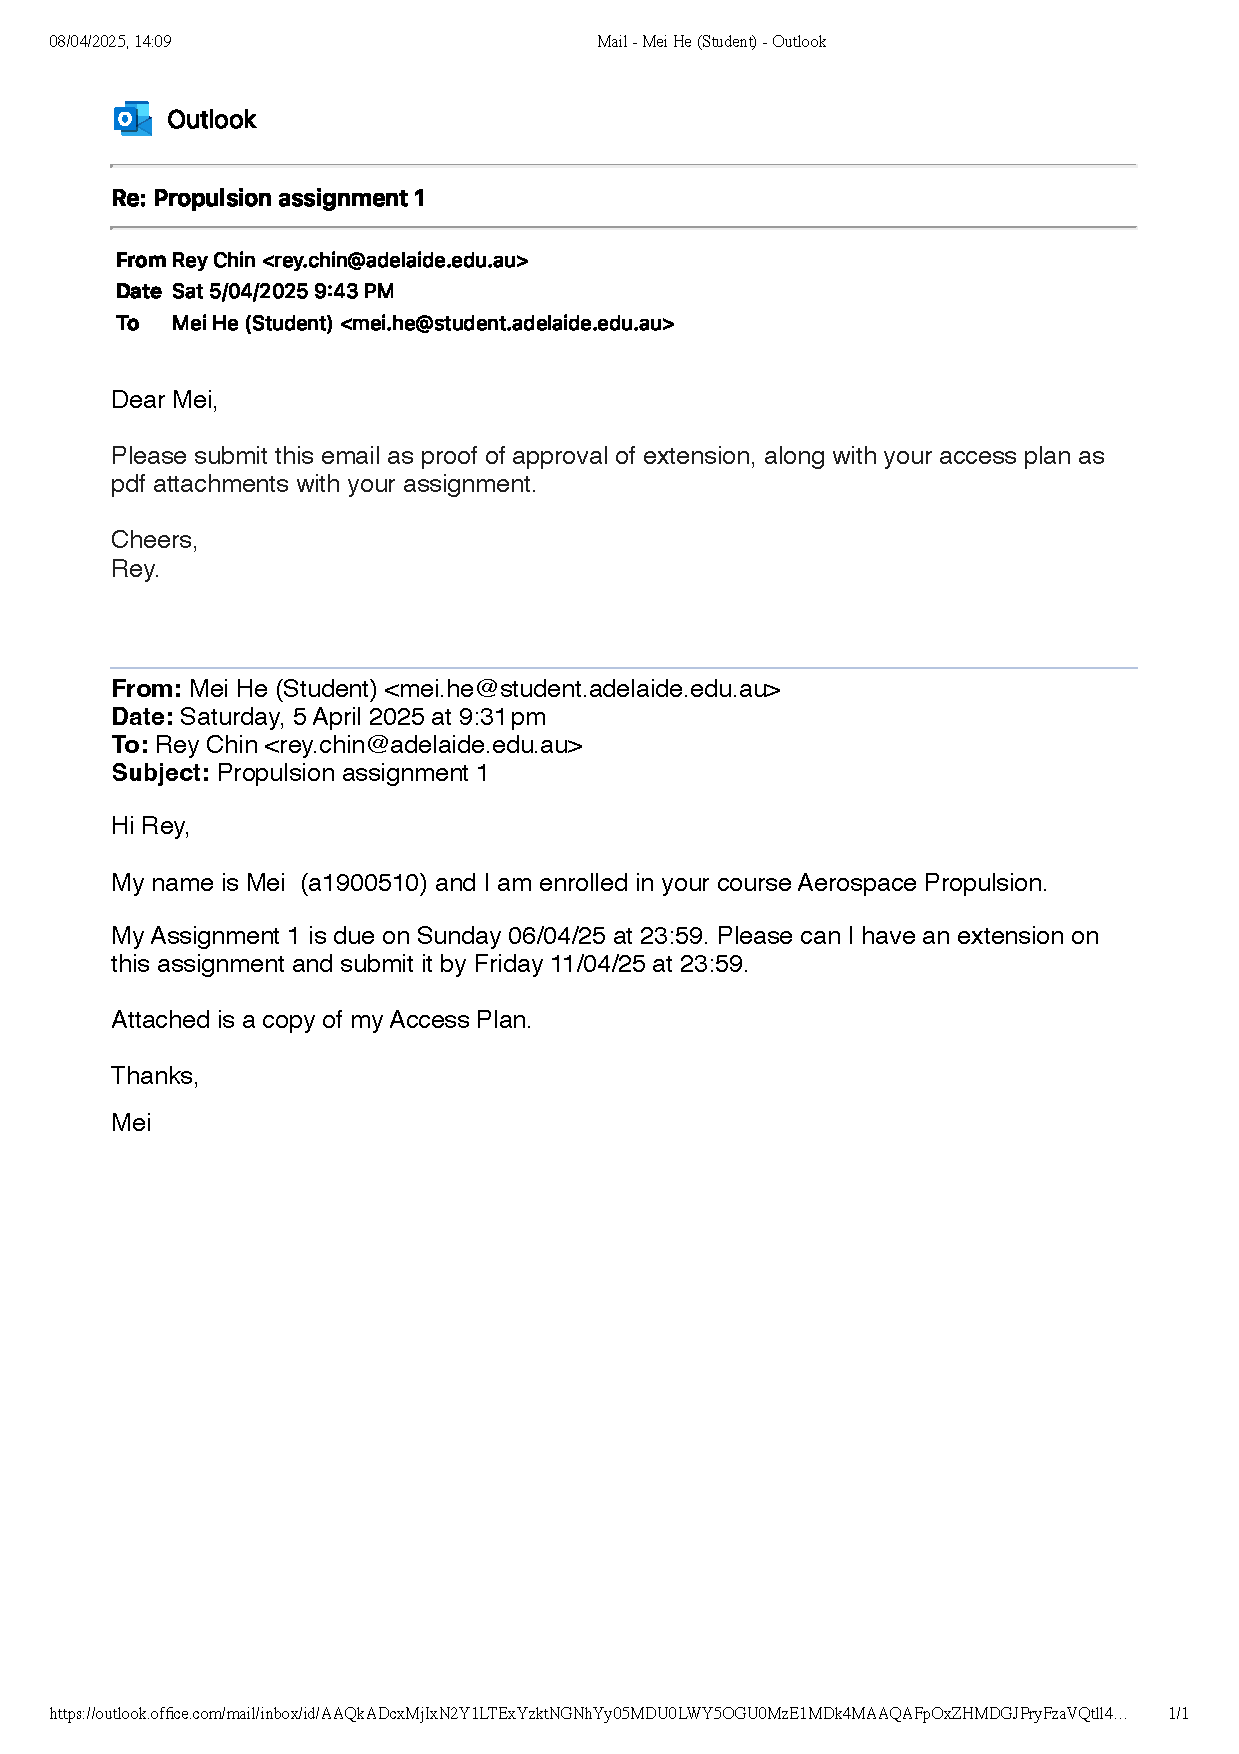
\includepdf[pages=-]{email_thread.pdf}}
\hypertarget{accessplan}{
\includepdf[pages=-]{MH_AP_Jan2024.pdf}
}

\end{document}


 